\chapter{Experimental Environments}

The experimenting environment is of most importance for technological evaluation. It is also impossible to find a configuration which can do both technologies justice. One can easily end up trapped by some technological limitation of a framework that one used or in the case of this thesis, confined by existing infrastructure provider. However, as the thesis is conducted under the company context, the limitations have to be accepted and taken into account. 

\section{Server in local machine}
Locally a virtual box running in Ubuntu 14.04 with 4 CPUs and 12G memory is installed on host machine which is a Macbook  Pro with 4 CPUs and 16G Memory. However, the application has to share the resource with database and load generator which is not at all a neat configuration. 

\section{Server running environment -  Cloud Foundry}
Cloud Foundry is an open source software bundle that allows you to run a polyglot Cloud Computing \ac{PaaS}. Initially it was developed as a Java \ac{PaaS} for Amazon EC2 by Chris Richardson, in 2009 acquired by SpringSource, which was then acquired by VMWare, then handed over to Pivotal.
The Cloud Foundry Foundation  \citep{Pivotal}  is now the maintainer of Cloud Foundry. More than 50 companies are members of this foundation, such as Pivotal, EMC, HP, IBM, Rackspace, SAP, or VMWare.
The Cloud Foundry PaaS is a multi-component automation platform for application deployment. It provides a scalable runtime environment that can support most frameworks and languages that run on Linux. It also contains many components that simplify deployment and release of microservices applications (for instance, Router, Loggregator, Elastic Runtime (\ac{DEA}), a message bus (NATS), Health Manager, Cloud Controller, etc.)

\subsection{Cloud Foundry at SAP}
Compared with other PaaS offerings, Cloud Foundry has some unique features: it has no limitation on language and framework support and does not restrict deployment to a single cloud.  It is an open source platform that one can deploy to run his apps on his own computing infrastructure, or deploy on an IaaS like \ac{AWS}, vSphere, or OpenStack. In SAP, it is first integrated with SAP Monsoon, then later shifted to Openstack and now hosted in \ac{AWS}. \\
There are two different landscape of Cloud Foundry in SAP. One is called "AWS live". In this landscape, applications run inside containers managed by Warden   \citep{Warden} containerization (a visualization technique providing isolation on operating system level, which is more efficient than virtual machines). The Warden containers including the applications running inside are managed by \ac{DEA} that also monitor the application health and provide the management interface to the Cloud Foundry platform.\\
The other landscape is called "AWS Canary". Instead of \ac{DEA}, each application VM has a Diego Cell   \citep{Diego} that executes application start and stop actions locally, manages the VM’s containers, and reports app status and other data to the \ac{BBS} \citep{BBS} and Loggregator. Instead of Warden, Garden \citep{Garden} is used as the containers to create and manage isolated environments. Diego architecture improves the overall operation and performance, for example supporting Docker containers.

\subsection{ Backing services , Service plans,and Scaling}
Services such as database, authentication form the core of a \ac{PaaS} offering. Cloud Foundry emphasizes on its flexibility in terms of backing services. It distinguishes managed services that obey the Cloud Foundry management APIs, and User-provided Services that serve as adapters to external services. In context of SAP, featured service like Hana database is offered along with other popular SQL and NoSQL databases. These services come with different plans, which define the size and capacity they are capable of offering. For example, PostgreSQL database has a service plan which is delivered in a docker container with predefined maximal number of connections. There are also other plans which provide PostgreSQL in dedicated VMs with different database sizes from extra small to extra large. \\
Service binding in Cloud Foundry is a simple way to tell the application to use a certain backing service. With frameworks like Spring cloud, database connector makes it extremely simple to enable the connection within application. In this thesis, as no extra frameworks is used, application parses the database information from the environment variable \textit{VCAP\_SERVICES} . \\
Since applications and its essential external components are loosely coupled in the context of Cloud Foundry, it leads to easy scalibility which consists the ultimate goals of cloud.  In short, everything is a service: The application, framework functionality (such as persistency), and of course external services to use or integrate with. A service has its own data store, can be implemented and deployed independently, and communicates with other services using lightweight mechanisms.  In this way, horizontal scaling of the system is supported. One can scale services up and down by adding or deleting service instances.

\subsection{Limitations}
As mentioned at the beginning of this chapter, it is impossible to have a perfect environment to conduct a evaluation of the performance of given technology. It is even harder in Cloud Foundry. \\
\subsubsection{Limitation of CPU resource}
\label{cpu limitation}
The first difficulty is to ensure that both applications obtain the equal computing resource. Easiest way is to have JAVA and node applications running on the same VM. However, in Cloud Foundry, applications are not confined to a single cloud. There is no way to secure a dedicated VM on which only the given applications are running. So if one doesn't know if application is running on the same node, one tries to at least make sure both applications have the same CPU allocated. As mentioned above, Cloud Foundry uses containerization which provides operating-system-level visualization instead of simulating bare computing hardware. This means multiple instances running in their respective containers share the same operating system. CPU shares instead of direct CPU time are first distributed. Each container is placed in its own cgroup. Cgroups make each container use a \textit{fair share} of CPU relative to the other containers \citep{CGroup}.This includes two layers of meanings. First, CPU shares are set aside for application according to the memory. Applications with larger amount of memory reservation receive more CPU shares. But does the applications have the same CPU resource when they occupy the same amount of memory? Not necessarily. The second step to designate CPU time is \textit{relative to the other containers}. The following table \ref{CPU time in Cloud Foundry} shows the CPU allocation for 3 applications running in the same VM. 
\begin{table}[h]
	\caption{Example: allocate CPU time in Cloud Foundry}
	\label{CPU time in Cloud Foundry}
	\renewcommand{\arraystretch}{1.2}
	\centering
	\sffamily
	\begin{footnotesize}
		\begin{tabular}{l l l l l }
			\toprule
			\textbf{Application Name} & \textbf{Memory} & \textbf{CPU Shares}& \textbf{CPU Percentage} }& \textbf{State}\\
			\midrule
		    A 	&	100	m & 10 & 20\%   & running\\
			B	&	200 m & 20 & 40\% & running\\
			C	&	200 m &	20 & 40\% & running\\
			\bottomrule
		\end{tabular}
	\end{footnotesize}
	\rmfamily
\end{table}

Nevertheless, this schema of CPU allocation only shows when all the applications are running. If application A now start idling, B and C will both get 50\% of the CPU resources. If only C is running, it gains whole 100\% of the computing power. Now you see why securing identical CPU resource for two applications deployed in Cloud Foundry is impossible. \\
\subsubsection{Limitation of database service}
Cloud Foundry backing services are very convenient to use but is not free of charge when one need a bit more performance. In this thesis, the docker container version of PostgreSQL is used owing to the fact that all other dedicated services cost. The database used in the thesis has a limited connections of 100 per service instance. Luckily,  with connection pooling one application barely needs so many connections. Nevertheless, it does set a threshold on how many instances the application can scale. Large number of scaling is not discussed in the thesis therefore the database is still chosen as default for the performance testing. \\

 \subsubsection{Limitation of proxy server}
 \label{haproxy}
Scalibilty certainly doesn't come for free. The minute system is under stress, the whole landscape of Cloud Foundry is facing challenge. During the thesis, a strange scenario has occurred: the total number of throughput in a minute lingers around 21,000 to 23,000 when the parallel requests reach a certain number. There must be a bottleneck somewhere. Is it because of how the application is implemented? Then the throughput should rise when more application instances are there to handle requests. However, no matter how many application instances are running to relieve the stress, the result stays the same.  The CPU usage of the application doesn't go beyond 20\%. The load is no more than a scratch on the application.\\
Is it because the database simply no longer has enough connection? We can try to give application an additional database. To scale the database is somehow more complicated than scaling the application. Instead of adding one instance to the existing application, another identical application is deployed to Cloud Foundry with its own database instance. The same route is mapped to the new application. Load balancer distributes the requests between two applications. As there are two database instance now, the database capacity is doubled. However, this also changes nothing. To absolutely rule out the limitation is database, the application is pushed to cloud without database at all as a simplest "Hello World" application. The limit of throughput persists. \\ 
Finally, after some searching into existing issues reported from other users, it turns out the bottleneck is in network. Cloud Foundry has a router written in Go, called Gorouter  \citep{Gorouter} which does routing and load balancing. The router performs perfectly and can handle 5,000 requests per second without a hiccup. Nonetheless, Gorouter is not the only thing standing between client and application. The requests coming outside of Cloud Foundry are secured HTTPS calls to keep sensible information from hackers while routes are not encrypted during load balancing. This means before the request is routed to the destination, another server has to terminate SSL and change HTTPS calls to HTTP. This task is accomplished by \ac{HAProxy} \citep{HAProxy} by the time the thesis is finished. HAProxy is never meant to be put in a productive Cloud Foundry landscape owing to its incapability of scaling. Every HAProxy can handle maximum 100 requests per second till its CPU consumption hits the celling. That is when it stops handling any more requests. In the current landscape, there are 4 HAProxy servers. Since they can not scale, it results in a network bottleneck where no more that 400 requests per second can be consumed. This is exactly why the strange scenario come into being. To overcome this restriction, either the proxy server should be changed into scalable ones, which is on the agenda of first quarter 2017 or keeping the connection to Gorouter alive and sending more requests in one decrypted connection. The latter choice is carried out in this thesis which is mentioned in \ref{load generator}.


\section{ Client running environments}
Where the client is running can influence greatly on the performance of the server. Do they share the same database? How great is the network latency? Do they share the same computing resource? To minimize all the influence to zero is next to impossible. Different approaches are discussed in the following. 

\subsection{Client in local machine}
Running server and client in the same physical machine kind of limited the network overhead. However, they consume the same computing resource and inevitably affected by other processes simultaneously operating in the same machine. One client instance won't be enough to generate load to stress application. Regardless, the moment one tries to scale the total of client applications, then it is competing resource with the actual application. This leads to tainted test results.  
\subsection{Client in Cloud Foundry}
Running the client in Cloud Foundry poses less network overhead for the request. Although requests still have to go through HAProxy to arrive at Gorouter despite the fact that client and server are under same domain or even running on the same node. Another convenience to run client on Cloud Foundry is that it is simple to scale. One client instance will have its limitation in sending parallel requests, but one can have as many instances as one needed. This is powerful and essential for this thesis. 

\section{Server and client configuration in the thesis}
\begin{figure}[h]
	\centering
	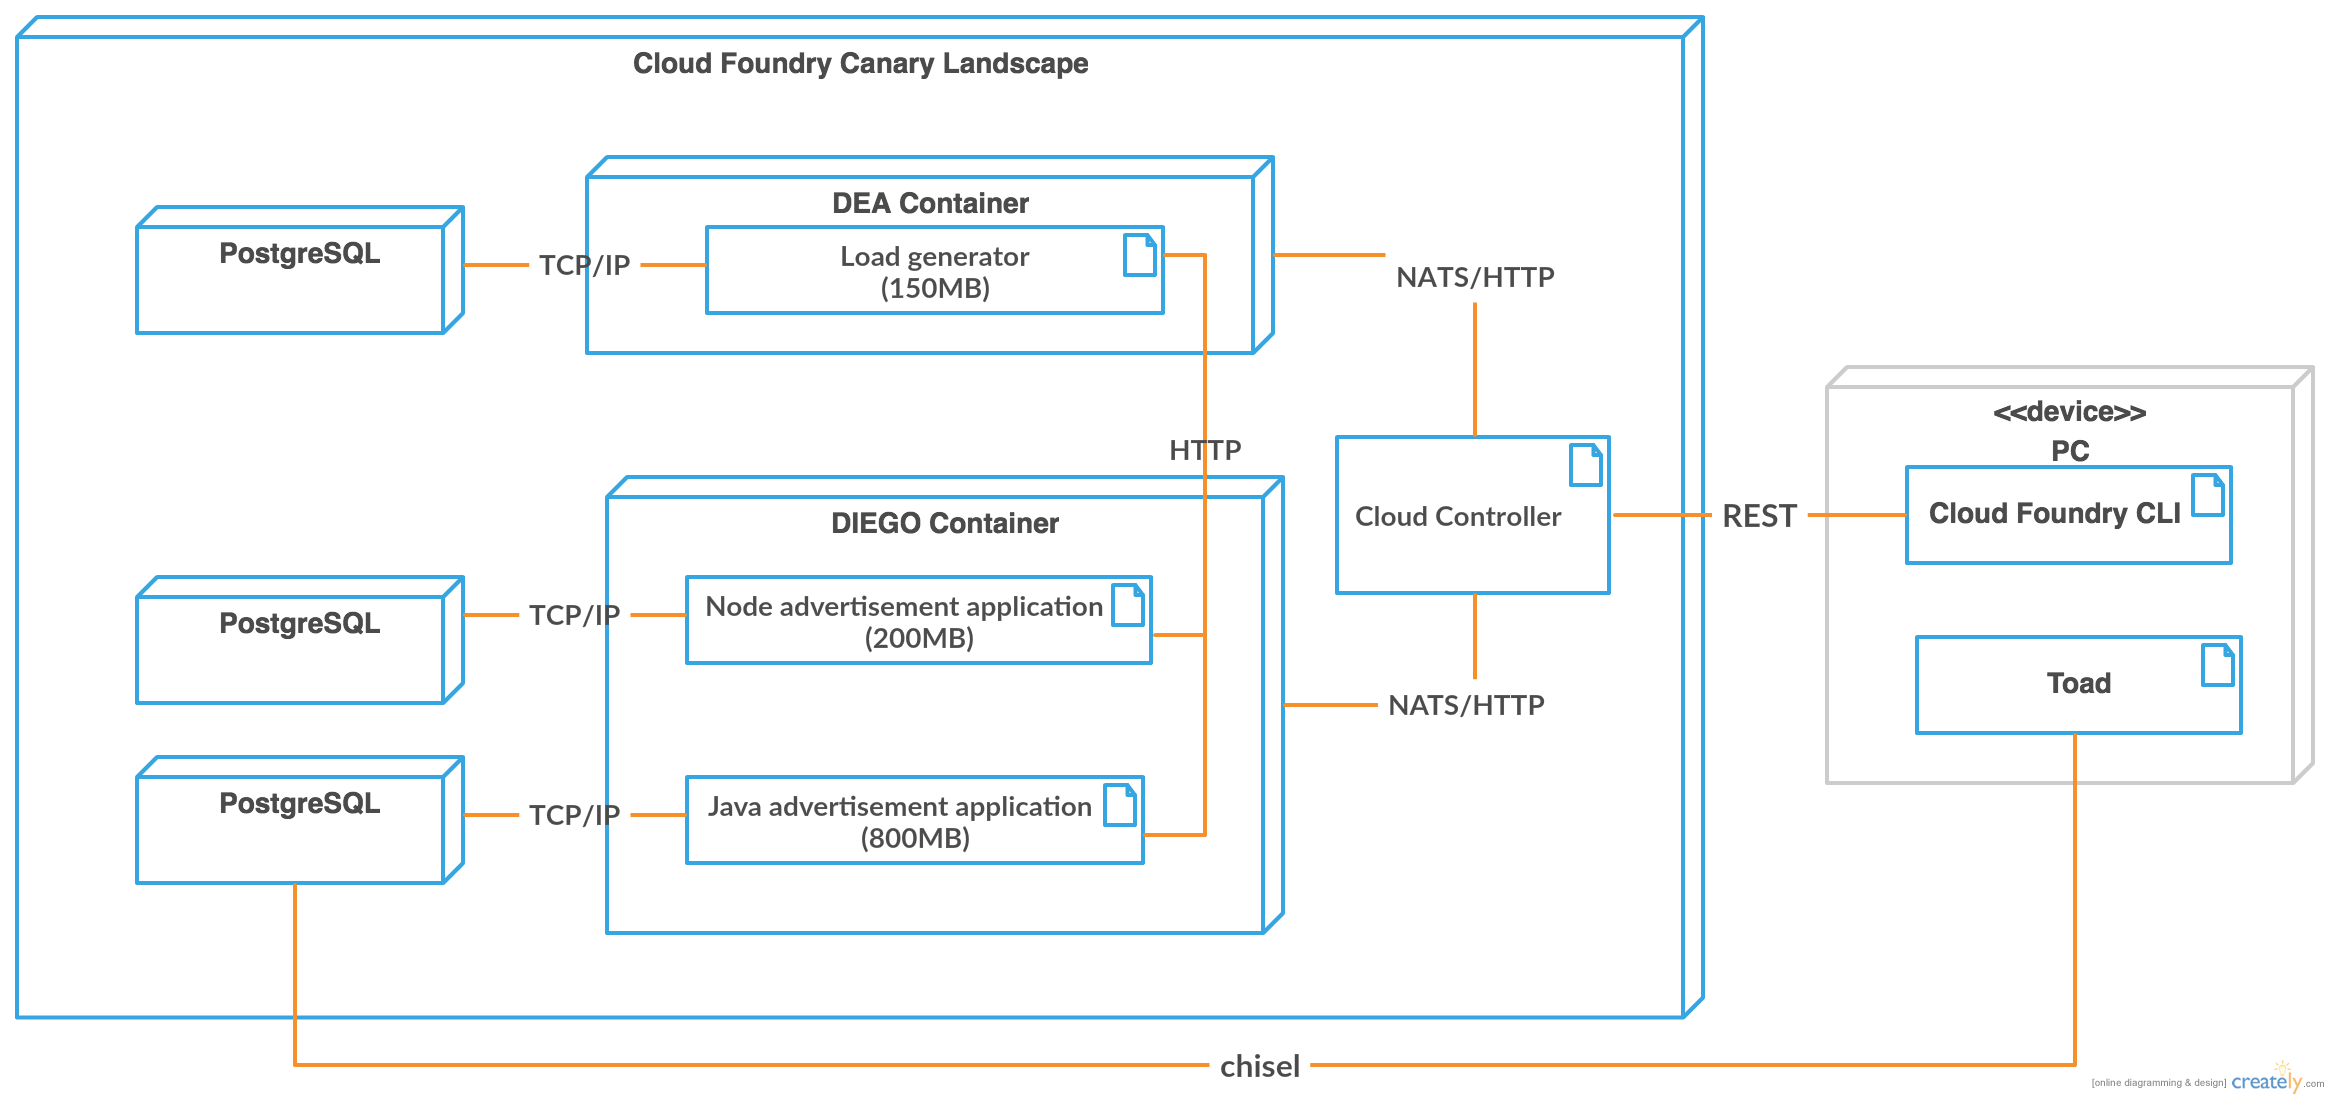
\includegraphics[width=14cm]{deployment_diagram}
	\caption{Deployment diagram for test environment}
	\label{deployment-diagram}
\end{figure}
With all the matters considered, figure \ref{deployment-diagram} shows the final setting of testing environment. First, both client and server are deployed in the same landscape in Cloud Foundry in order to minimize possible network overhead. Second, to avoid the scenario that load generator is running in the same node as the applications, the client and server are deployed into different containers. Clients are in DEA while applications are deployed to Diego. In addition, separate PostgreSQL database services are assigned to applications so that the load on the database is distributed. To retrieve data from database, chisel is used to bring TCP tunnel over HTTP, so that Toad extension on local machine can access the test results. Finally, through Cloud Foundy CLI, requests on application health is made and CPU and memory consumption information is gathered. \\
Another thing to pay attention to is how much memory the applications are allocated. For Java application, 800MB memory is set aside. As mentioned in \ref{memory}, it turns out Java needs about 300MB. However, since Java relies heavily on CPU shares allocated to it, more memory is alloted to ensure it has enough CPU even in a crowded node. On the contrary, Node.js application is given 200MB for the reason that it is single-threaded and more memory doesn't help it gain more computing resource. For the sake of not running into situation of not enough memory due to operational overhead in application such as garbage collector, memory is given quite generously to both applications.  



